\section{Scheduling}
I a program with concurrency, the exact order processes are executed is not completely specified. Different methods can be used to ensure that the correct task is running at the correct time. It is possible to use semaphores to restrict one process to use any shared data at a time, or a message can be used to make a process wait for a computation to finish. These methods, however, does not stop processes from interleaving, which makes it possible for processes to block another process from accessing a shared resource when it is needed. Some processes can be more important than others. If a non-important process blocks a safety-critical process, because they use the same shared resource, it can make the critical process fail, and in a worst case scenario cause harm to someone. To stop this from happening, we need scheduling.

Scheduling ensures that a concurrent program produces the expected outcome in all cases, and that it is correct with respect to timings. A scheduler has two main parts: 

\begin{itemize}
\item A scheduling algorithm that consists of a set of rules that order the use of system resources.
\item An analyzer that predicts the systems worst-case behavior.
\end{itemize}

The worst-case behavior will be compared to the deadline of the system, to check whether it is acceptable or not. If the programs worst-case behavior does not fulfill the time constraints of the deadline, a hard real-time system will not be able to be scheduled. A soft real-time system, however, might be able to stop unnecessary processes in time of need, to make sure that the critical part of the program makes the deadline.

Real-time scheduling algorithms put emphasis on the timing requirements of each process, even if this means a lower overall system performance. This is in stark contrast to the general-purpose scheduling algorithms, such as the Linux scheduler. These general-purpose schedulers focus on fairness, efficiency and throughput. Meaning that every process must at some time get processor time, the scheduler algorithm must use as few resources as possible and that the general performance must be as high as possible.

Some of the more common concepts used iin real-time schedulers are Cyclic Executive and Task-Based Scheduling (ex. FPS and EDF), these all follow the Simple Process Model. This Simple Process Model describes a set of properties that a program must comply with, if these  schedulers can be used.

These properties are as follows\cite{simpleprocessmodel-slides}:

\begin{itemize}
\item The application has a fixed set of processes
\item All processes are periodic with known periods
\item The processes are independent of each other
\item All processes have deadline equal to their period
\item All processes have a fixed worst-case execution time
\item All context-switching costs etc. are ignored
\item No internal suspension points (e.g., delay or blocking I/O)
\item All processes execute on a single CPU
\end{itemize}

These properties cannot always be met in real-world systems. Specifically, processes can be sporadic rather than periodic, deadlines can be longer or shorter than the period, a system may be overloaded in situations where computational demand exeeds the system capacity. In order to define these schedulers, we assume that a system complies with the Simple Process Model.

\subsection{Cyclic Executive}
The Cyclic Executive scheduler expects a fixed set of periodic tasks. The idea of the scheduler is to create a static schedule that includes all tasks in such a way that all tasks always finish within their deadline. The Cyclic Executive scheduler contains synchronization points where the task execution aligns itself with a time reference, usually a real-time clock or an interrupt. These synchronization points are called minor cycles, these usually chosen to be the period of the shortest task. The Cyclic Executive scheduler also has another type of cycle, the major cycle. The major cycle is the complete table of tasks that should be scheduled, this also means that all tasks must run in every major cycle.

\begin{figure}[hbtp]
\center
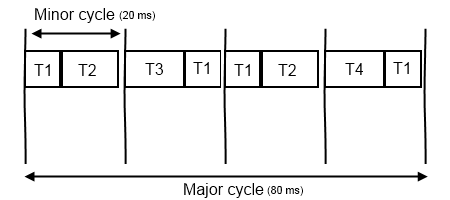
\includegraphics[width=\textwidth]{img/cyclic-exec.png}
\caption{An example of the Cyclic Executive scheduler} 
\label{fig:cyclic-exec} 
\end{figure}

An example of a Cyclic Executive scheduler is shown on \autoref{fig:cyclic-exec}, here we have four tasks, T1 has a period of 20 ms, T2 has a period of 40 ms, T3 and T4 both has a period of 80 ms.
The Cyclic Executive scheduler is very easy to implement, but it is difficult to construct and maintain.

\subsection{Task-Based Scheduling}
There will be a description of Task-Based Scheduling here.
